\begin{figure}
  \centering
  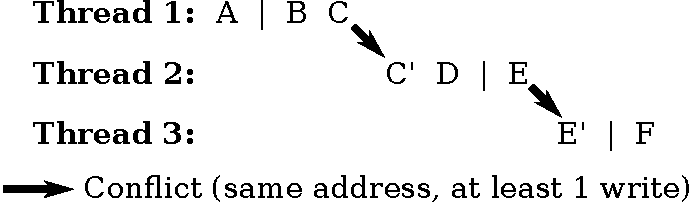
\includegraphics[width=.55\linewidth]{PersistencyModels/propagation.pdf}
  \caption{\textbf{Epoch persistency persist order.} Persistent memory order is enforced through persist barriers (shown as `` $\vert$ ") and access conflicts.  Access A is ordered by transitivity before access F.  If these accesses are persists they may not be reordered with respect to the recovery observer.  This order is enforced even if accesses are to the volatile address space.  Access B is concurrent with all shown accesses from threads 2 and 3, while access D is concurrent with accesses from thread 1.}
  \label{fig::EpochPersistencyPropagation}
\end{figure}
